
Atmospheric neutrinos have the potential to resolve the neutrino mass
hierarchy via matter-enhanced oscillation within the Earth.  Resonant
oscillation occurs either for neutrinos in the case of the normal
hierarchy, or antineutrinos for the inverted hierarchy.  Determination
of the hierarchy requires measurement of the energy and direction of
Earth-crossing atmospheric neutrinos with energies in the range of 2
to 10~GeV. Massive detectors ($\gtrsim$Mton) are required to obtain
sufficient signal statistics within a few years of operation.
Existing proposals use either water Cherenkov (PINGU, ORCA, HyperK),
liquid Argon TPC (LBNE, LBNO), or magnetized iron calorimeter (INO)
detectors.  Discrimination of neutrinos from antineutrinos enhances
hierarchy sensitivity.  Hierarchy determination has some dependence on
the oscillation parameters, in particular ${\Delta}m^2_{31}$, but is largely
insensitive to the 
Earth density
profile.  Primary concerns are detector properties such as total mass,
energy resolution, and angular resolution.

\subsection{Signature of the neutrino mass hierarchy}\label{atm:sign}

The two possible neutrino mass hierarchies predict distinctly
different oscillation probabilities for Earth-crossing neutrinos.  Due
to interactions with electrons within the Earth, resonant flavor
conversion occurs at a specific pattern of neutrino energies and
Earth-crossing paths.  This resonant conversion only occurs for
neutrinos in the case of the normal hierarchy, while only for
antineutrinos for the inverted hierarchy.  A detector capable of
discriminating $\nu$ interactions relative to $\overline{\nu}$ needs
only to demonstrate for which state the resonance occurs.  Detectors which
only distinguish neutrino flavor rely on the intrinsic difference in
the atmospheric flux between $\nu$ and $\overline{\nu}$ as well as
differences in interaction cross-sections to discriminate the
hierarchy.


\begin{figure}[tp]
\begin{center}
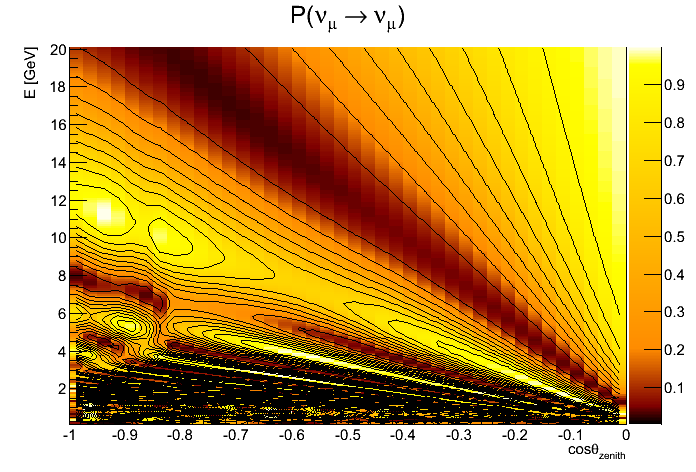
\includegraphics[width=7.5cm]{KBL/osc_MuMu_NH_10lyr.png}
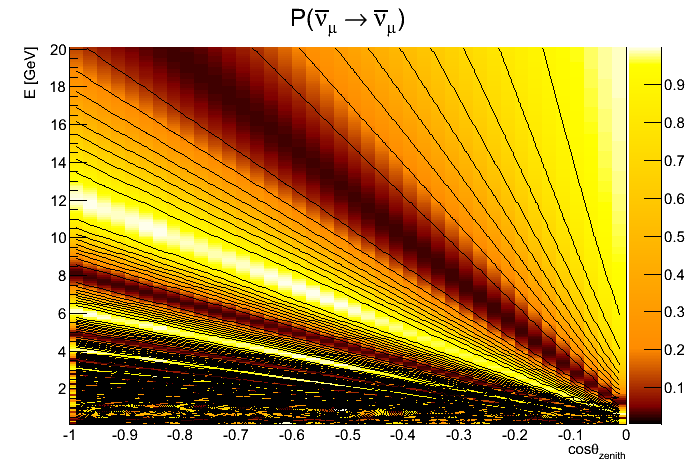
\includegraphics[width=7.5cm]{KBL/osc_AntiMuMu_NH_10lyr.png}
\caption{The estimated oscillation survival probability for
  Earth-crossing $\nu_{\mu}$ (left) and $\overline{\nu}_{\mu}$
  (right), assuming the normal neutrino mass hierarchy.  Resonant
  oscillation in the mantle is most significant in the region
  $\sim$6~GeV and cos$\theta_Z\simeq -0.7$, as indicated by the difference between the two panels.  For the inverted hierarchy,
  the resonance occurs for $\overline{\nu}_{\mu}$ instead of
  $\nu_{\mu}$.}
\label{fig:atmoNuProb}
\end{center}
\end{figure}

Resonant oscillation of Earth-crossing atmospheric neutrinos has been
extensively examined~\cite{atm:Petcov1998, atm:Akhmedov2008,
atm:Akhmedov}.  Oscillation probabilities are commonly presented as
Earth {\em oscillograms}, which show probabilities as a function of
neutrino energy and zenith angle $\theta_{Z}$.\footnote{Downward-going
neutrinos have cos$\theta_{Z}$=1, while upward-going neutrinos which
have crossed the Earth's core have cos$\theta_{Z}$=-1.}
Fig.~\ref{fig:atmoNuProb} shows the calculated oscillation
probabilities assuming the normal hierarchy.  

 Assuming a 1~Mton detector,
$\sim$4000 muons per year are generated in the energy range of 2 to
10~GeV.  Fig.~\ref{fig:atmoMuRates} shows the rate of muon production
per Mton-yr assuming the normal hierarchy.  The major feature of the
hierarchy is the resonant excess of muons at $\sim$6~GeV and
cos$\theta_Z\simeq -0.7$.  The intrinsic $\nu$/$\overline{\nu}$ ratio of
$\sim$1.3 in the resonance region provides an observable signal of the
hierarchy, even for a detector insensitive to muon charge.

\begin{figure}[tbp]
\begin{center}
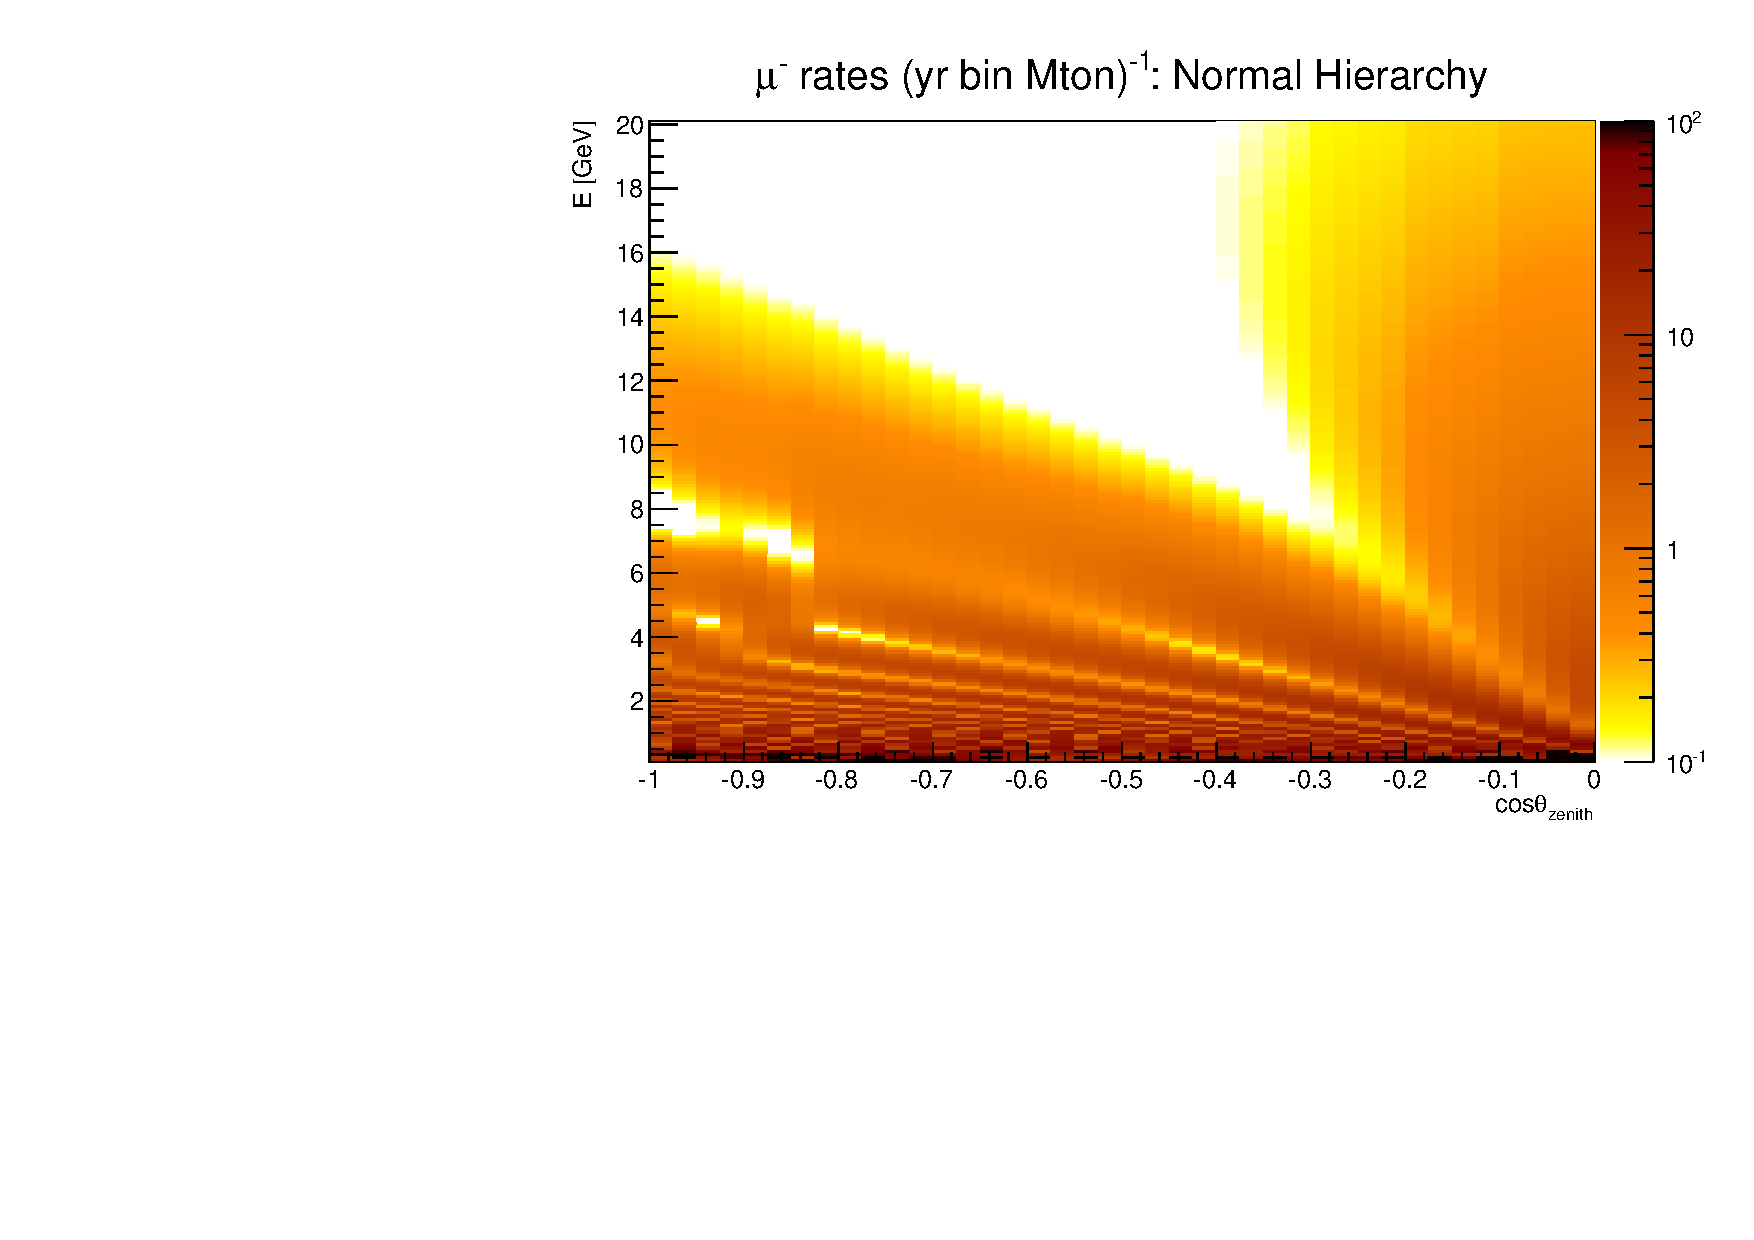
\includegraphics[width=7.5cm]{KBL/muRates_NH_MtonYr.pdf}
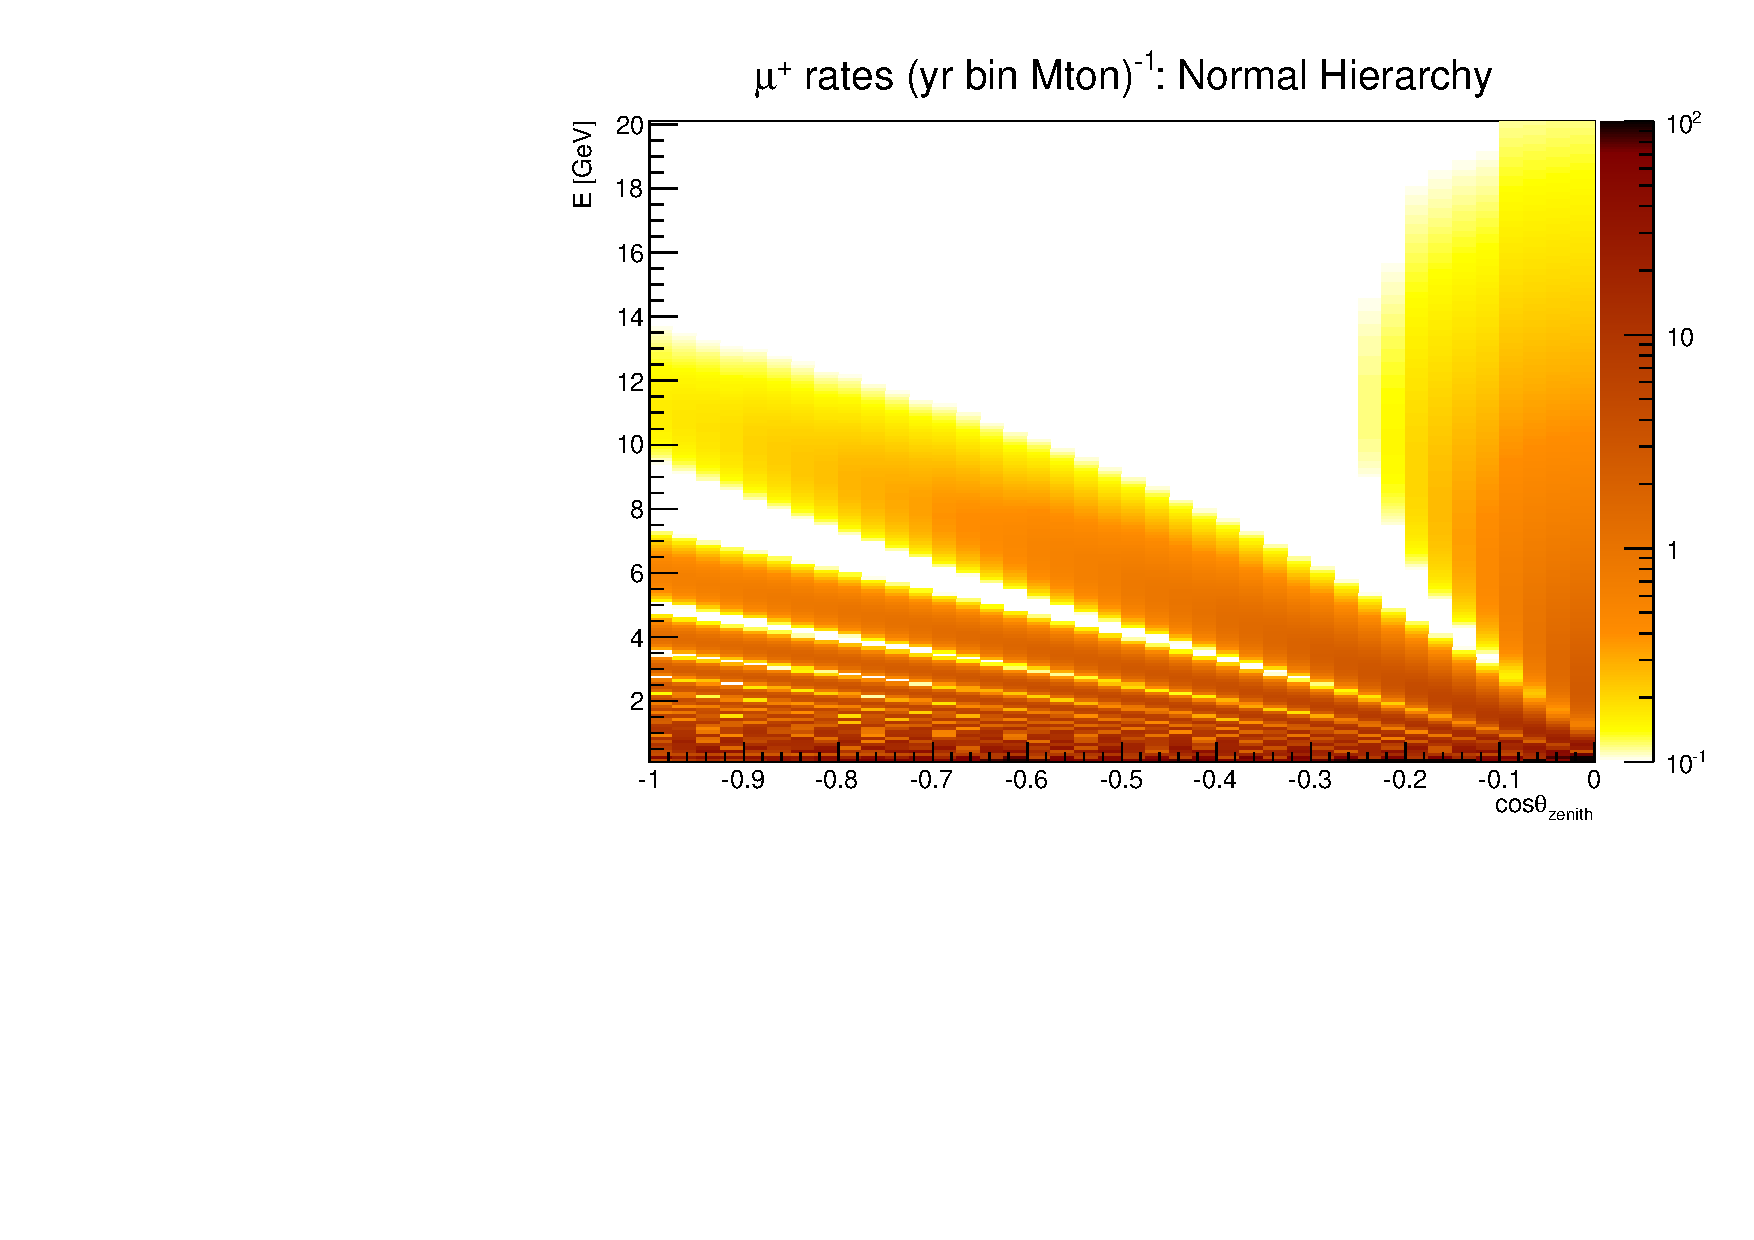
\includegraphics[width=7.5cm]{KBL/antiMuRates_NH_MtonYr.pdf}
\caption{The estimated rate of atmospheric neutrino generated $\mu^-$
  (left) and $\mu^+$ (right) per Mton-yr, assuming the normal neutrino
  mass hierarchy.  The rate is shown as a function of the incoming
  neutrino energy and direction.  The hierarchy is most significantly
  visible as a resonant enhancement of $\mu^-$ at $\sim$6~GeV and
  cos$\theta_Z\simeq -0.7$.  For the inverted hierarchy, the resonance
  occurs for $\mu^+$ instead of $\mu^-$.  For a detector insensitive
  to muon charge, the hierarchy produces a change in the rate
  according to the intrinsic $\nu$/$\overline{\nu}$ ratio of $\sim$1.3
  in this resonance region.}
\label{fig:atmoMuRates}
\end{center}
\end{figure}

Sensitivity to the hierarchy is primarily driven by how well the
initial neutrino energy and direction can be determined.  It is clear
that as the energy resolution increases beyond a few GeV, the
resonance feature is obscured.  Intrinsic resolution is introduced by
the kinematics of the outgoing muon and nuclear effects for GeV $\nu$
interactions.   Of concern is the uncertainty in
${\Delta}m^{2}_{31}$, which has the strongest correlation with the
predicted oscillation pattern for muon-charge insensitive detectors.

\subsection{Proposed Experiments}\label{atm:expts}

\subsubsection{INO and MIND}

The India-based Neutrino Observatory (INO) will be located in the Bodi-West Hills in Pottipuram village
near Bodinayakanur in the Tamil Nadu State, with an overburden of about
1.3 km~\cite{atm:Dighe}.  Three
detector modules will form a 50-kT magnetic iron calorimeter.   The prominent features of the INO detector are its
capability of determining the charge and momentum of the the muon in
the charged-current interaction of an atmospheric muon
(anti-)neutrino, and the energy of the hadronic shower.  These
features would allow for discrimination between neutrinos and
anti-neutrinos as well as their energy.

MIND~\cite{nonus:LBNO_LOI} is a proposed 25~kT magnetized
iron-scintillator calorimeter, to be constructed in conjunction with
the European long-baseline effort in an underground lab in
Pyh\"asalmi, Finland. Its sensitivity to atmospheric neutrino
oscillations can be inferred from the INO numbers below. 

From a GEANT4-based simulation, the energy resolution of the hadronic
component, $\sigma/E$, is about 40\% for hadronic energies greater
than 4 GeV and is quite independent of the zenith angle of the
incident (anti-)neutrino.  The efficiency of correctly identifying the
charge of a track is better than 95\% for cos$\theta>0.35$ and
momentum greater than 1 GeV.  For momentum greater than 1 GeV, the
momentum resolution, $\sigma_p/p$, is better than 22\% and the
resolution in $\cos\theta$ is better than 0.045 for for
$\cos\theta>0.35$.


For sin$^2(2\theta_{13})$=0.1, the hierarchy can be resolved at 2
(2.7) standard deviations with 5 (10) years of running. The
sensitivity is limited by statistics. 

Civil construction for INO began in February 2013.  The first three detector
modules will be installed and commissioned in the underground
experimental hall by 2017. According to the schedule presented in Ref.~\cite{atm:Dighe},
excavation will take 1.5 years for a 2-km-long 7.5-m-wide tunnel,
which is quite an aggressive schedule when taking uncertainties in the
geotechnical conditions into account.

\subsubsection{PINGU}

Precision IceCube Next Generation Upgrade (PINGU) is a proposed
multi-megaton detector to be located below the dust layer in the inner
core of the existing IceCube and DeepCore detectors.  PINGU consists
of closely separated vertical strings of Digital Optical Modules
(DOMs) for detecting atmospheric neutrinos with energies down to a few
GeV.  In this configuration, IceCube and DeepCore serve as vetoes for
rejecting cosmic-ray muons both online and in the offline analysis.  The
DOM-to-DOM spacing is shorter than that of DeepCore.  The design
of the DOM is taken to be the one used in DeepCore.  The trigger
efficiency is expected to be much higher at lower energies for PINGU
than for DeepCore. 
The cost of constructing PINGU is about \$10 M for start up and \$1.25 M per string based on the 
IceCube experience.

\paragraph{Sensitivity}\label{atm:PINGUsen}

The sensitivity
for determination of the mass hierarchy by PINGU has been
estimated both by proponents of the experiment~\cite{atm:pingu} and
independently~\cite{atm:Winter}, as shown in Figs.~\ref{PINGU:senown} and~\ref{PINGU:sen}, respectively.  
According to
the proponents, PINGU can achieve a sensitivity of $\sim 2.1$-$ 3.4 \sigma$ per year of data taking, resulting in a $3 \sigma$ 
discrimination between the normal and inverted hierarchies 
 by 2020, assuming initial deployment in 2016/17.  
 Details on the underlying assumptions and statistical techniques used to evaluate the sensitivity are somewhat limited at this stage, although a more detailed  Letter of Intent is in preparation~\cite{atm:pc}.  
The conclusions of Ref.~\cite{atm:Winter} are more modest, presumably because of differing assumptions in detector performance or statistical methodology.  Ref.~\cite{atm:Winter} points
out the complementarity between PINGU and the current accelerator and
reactor oscillation experiments (\NOvA, T2K, Daya Bay, RENO, Double
Chooz). 
As identified in Ref.~\cite{atm:Winter}, the key factors
influencing the experimental sensitivity are the current uncertainty
on $\Delta m^2_{31}$, the total active detector mass, energy
threshold, energy and 
angular resolution, and mis-identified cascades.  The existing studies
have not incorporated possible muon charge discrimination via
inelasticity of the neutrino interaction. %

\begin{figure}[bp]
\begin{center}
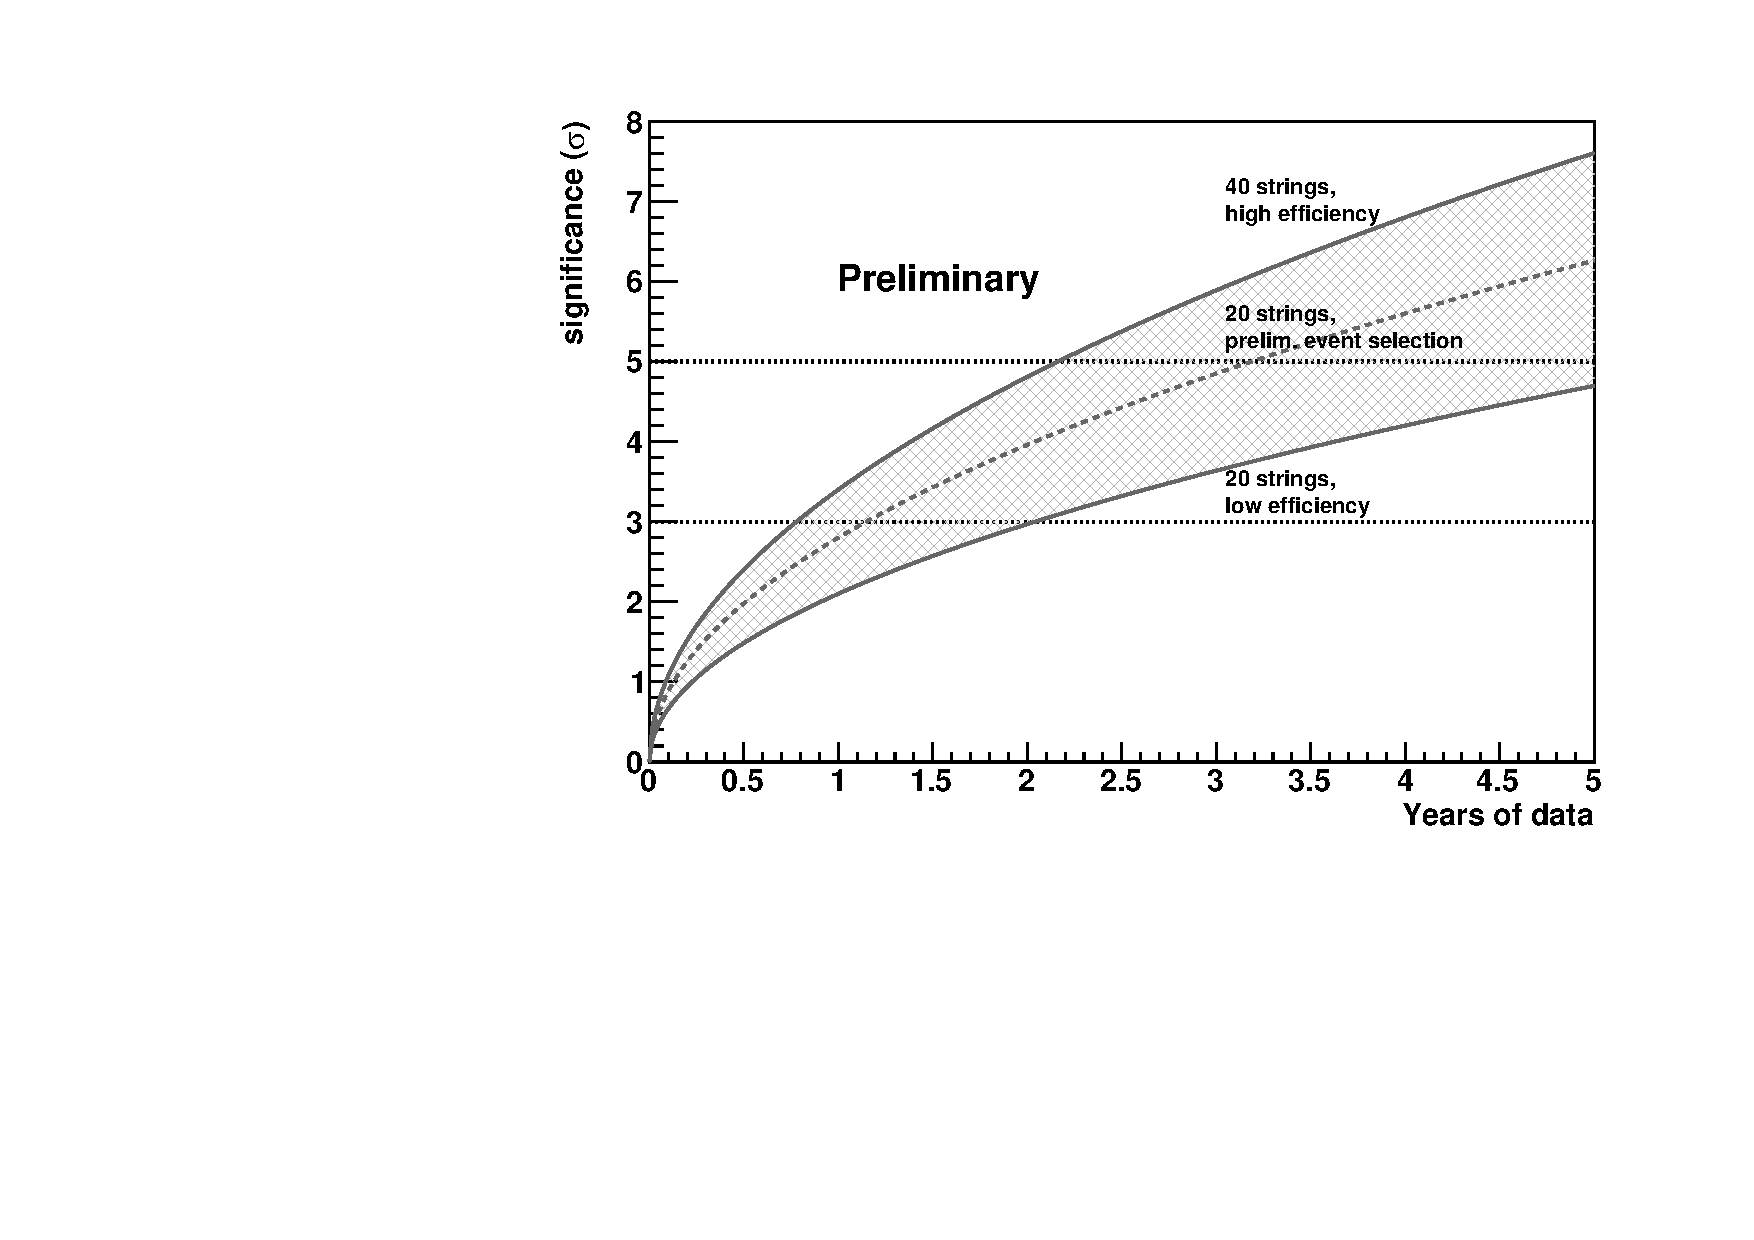
\includegraphics[width=0.6\textwidth]{KBL/pingu_nmh_sensitivity.pdf}
\caption{Significance of determination of the mass hierarchy using
PINGU as a function of run time, for different detector configurations, by the proponents of the experiment~\cite{atm:pingu}.  }
\label{PINGU:senown}
\end{center}
\end{figure}
\begin{figure}[tbp]
\begin{center}
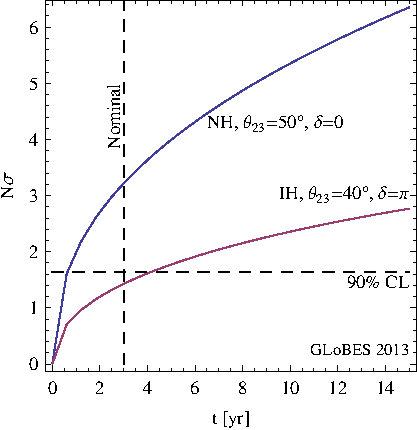
\includegraphics[width=0.52\textwidth]{KBL/atm_expplot.pdf}
\caption{Significance of determination of the mass hierarchy using
PINGU as a function of run time, for the best and worst case of the
true oscillation parameters, from an independent study~\cite{atm:Winter}.}
\label{PINGU:sen}
\end{center}
\end{figure}


It will take 1.5 years to procure and ship the detector components to
the South Pole.  Installation of all strings is expected to complete in
2-3 years.  If the proposal is submitted to the funding agencies in a
year, the full PINGU detector could be deployed by 2020.  Note that PINGU
can begin taking data as PMT strings are installed, slowly reaching
the full target mass by 2020.

Besides having relatively poor energy and directional resolutions, 
lack of charge determination and minimal particle identification 
could be an issue in achieving the scientific goals. 
Of primary concern is whether PINGU can achieve the required detector
performance characteristics.  These concerns with detector performance may be
mitigated by improvements in detector design, or even with incremental
extension of the detector after initial data has been obtained.


\subsubsection{ORCA}

Oscillation Research with Cosmics in the Abyss (ORCA) is a proposed
dense instrumentation of the central region of the KM3NeT detector in
the Mediterranean Sea~\cite{atm:Coyle}.  In principle, this is similar
in concept to PINGU, except the target is water instead of ice.  Funding of 40M Euros for KM3Net phase 1 has been secured, and 50-70
lines of sensors are expected to be ready for deployment by the end of
2016.  This comprises a total of 1200 pressure-vessel sensor modules,
each containing 31 3'' photomultiplier tubes.

\subsubsection{Hyper-Kamiokande}

Hyper-Kamiokande (HyperK) is a proposed multi-purpose water Cherenkov
detector, described in detail in Section~\ref{s:nonus}. 
The detector is based on well-known technology, and
is primarily a scale up of the existing Super-Kamiokande detector.  In
this respect, the expected performance in event reconstruction and
particle identification in the sub-GeV region is well-characterized.
The detector is  sensitive to and can discriminate both muons
and electrons.  However, it will have limited capability to determine
the sign of the lepton generated by the neutrino charged-current
interaction.

With excellent particle identification, HyperK can tackle the mass hierarchy
problem using both disappearance of muon neutrinos and appearance of
electron neutrinos. 
The expected statistical significance in settling the mass hierarchy of HyperK
is presented in Fig.~\ref{HyperK:sen}.
For sin$^2\theta_{23}=0.5$ and sin$^22\theta_{13}=0.1$, the wrong hierarchy
could be ruled out at almost three standard deviations with about five years of running.  
The discriminating power is weakly dependent on the value of the CP-phase 
$\delta_{CP}$.  Qualitatively, a small $\delta_{CP}$ will yield better discrimination 
for a given value of sin$^2\theta_{23}$.

\begin{figure}[tp]
\begin{center}
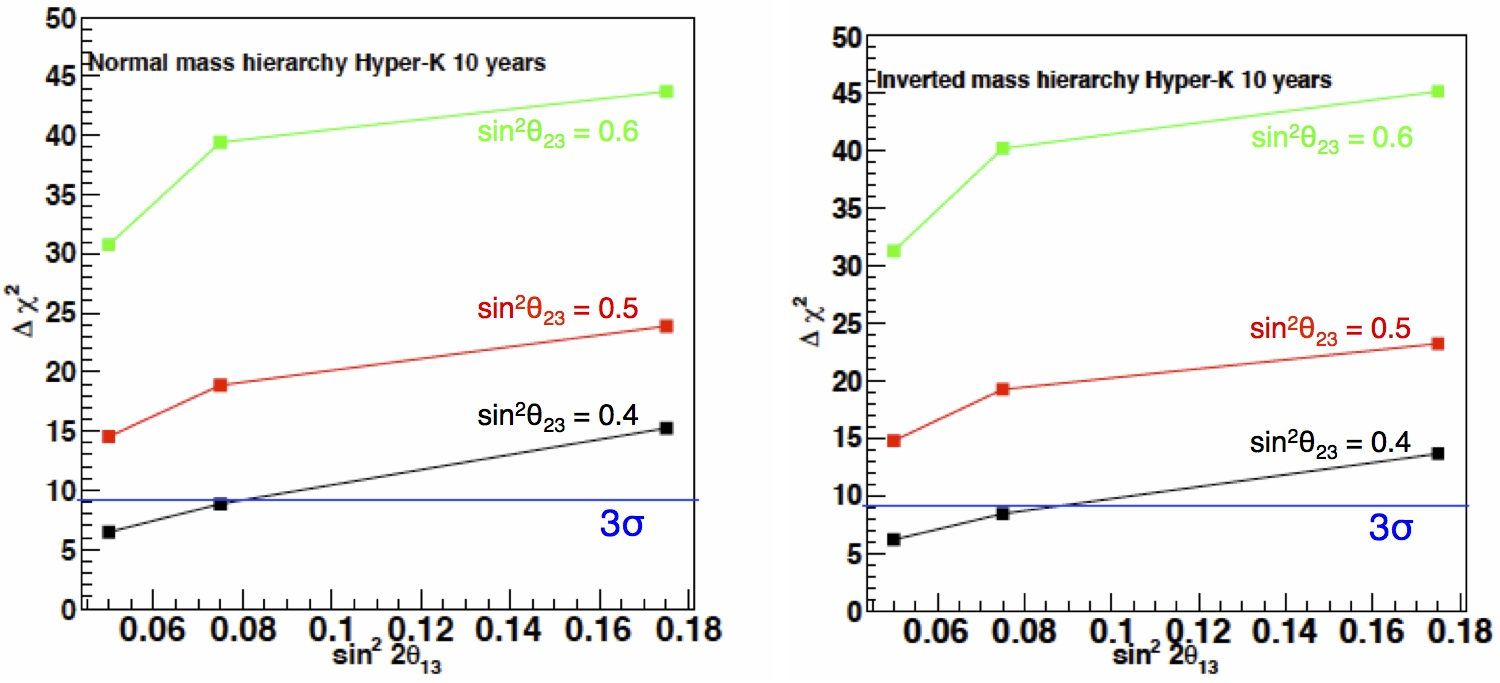
\includegraphics[width=0.95\textwidth]{KBL/HyperK_sensitivity.jpg}
\caption{Significance of discriminating the mass hierarchy when the true hierarchy is (Left) normal and (Right) inverted, as a function of sin$^22\theta_{13}$ and sin$^2\theta_{23}$, after 10 years of operation of HyperK~\cite{nonus:HyperK}.}
\label{HyperK:sen}
\end{center}
\end{figure}

In January 2013, HyperK was included in the future plan of
KEK~\cite{atm:Nakaya}. If funded, the project would start in JPY2016,
with the two-year construction of access tunnels beginning in
2016. Excavation of the underground cavern is expected to start in
2018 and beneficial occupancy would take place in 2021. Operation of
the HyperK detector modules would start in January 2023.
The main concern with HyperK is cost, which is estimated at  
\$500-700M (US).  It is unclear if Japan will have sufficient funding for
this experiment.  Given the drive for liquid argon-based long-baseline
accelerator programs in both the US and Europe, it is unlikely that
foreign partners will contribute significantly to the cost.


\subsubsection{Atmospheric neutrino experiments using liquid argon detectors}

Besides providing excellent particle identification, 
liquid-argon detectors are superior to iron-scintillator calorimeters, water Cherenkov
detectors, or ice-based detectors in energy and angular resolutions over the energy
range of MeV to multi-GeV.  
Furthermore, since the energy of the hadronic component of the charge-current
interaction is measured, the energy of the incident (anti-)neutrino can be determined. 
One could even imagine magnetizing a large liquid-argon detector for charge
discrimination. Thus, liquid-argon detectors could be an ideal tool for addressing
the mass hierarchy problem with atmospheric neutrinos. 

Assuming the energy resolution to be $\sqrt{(0.003)^2+(0.15)^2/E_{had}}$ 
for hadronic showers, 0.01 for charged leptons in the GeV range, and the angular 
resolution to be 0.03 (0.04) rad for electrons (muons or hadronic
showers), an estimated 
sensitivity in delineating the mass order as a function of
sin$^22\theta_{13}$ and  
sin$^2\theta_{23}$ for an exposure of 250 kT-yr is given in
Fig.~\ref{LAr:sen}~\cite{atm:LAr}. This exposure corresponds to: 25
years of operation of a Phase-I sized LBNE detector; 7.5 years of the full-scale 34-kT detector (either would need to be located underground); 12.5 years of Phase I of
LBNO-GLACIER; and only 2.5 years of the full GLACIER detector. Discrimination power of over
$3\sigma$ for the neutrino mass hierarchy seems achievable using liquid argon detectors. 


\begin{figure}[t]
\begin{center}
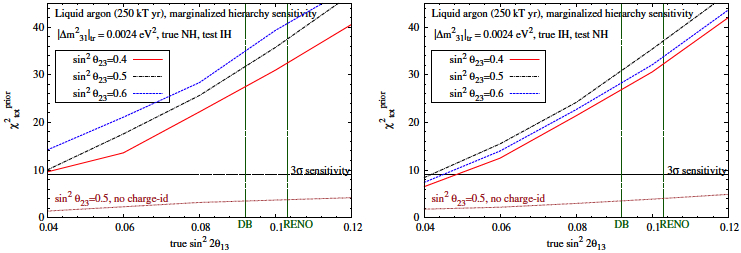
\includegraphics[width=0.95\textwidth]{KBL/LAr_sensitivity.jpg}
\caption{Significance of discriminating the mass hierarchy as a function of sin$^22\theta_{13}$ and sin$^2\theta_{23}$ after an exposure of 250 kT-yr for liquid-argon detectors~\cite{atm:LAr}.}
\label{LAr:sen}
\end{center}
\end{figure}





























